\documentclass[a4paper,12pt]{extarticle}
\usepackage[utf8x]{inputenc}
\usepackage[T1,T2A]{fontenc}
\usepackage[russian]{babel}
\usepackage{hyperref}
\usepackage{indentfirst}
\usepackage{listings}
\usepackage{color}
\usepackage{here}
\usepackage{array}
\usepackage{multirow}
\usepackage{graphicx}
\usepackage{algorithm}
\usepackage{algpseudocode}
\usepackage{caption}
\usepackage{pdfpages}
\usepackage{tikz,mathpazo}
\usepackage{graphicx,amssymb,amstext,amsmath,newtxmath}
\usetikzlibrary{shapes.geometric, arrows}
\renewcommand{\lstlistingname}{Программа} % заголовок листингов кода

\bibliographystyle{ugost2008ls}

\usepackage{listings}
\lstset{ %
extendedchars=\true,
keepspaces=true,
language=C,						% choose the language of the code
basicstyle=\footnotesize,		% the size of the fonts that are used for the code
numbers=left,					% where to put the line-numbers
numberstyle=\footnotesize,		% the size of the fonts that are used for the line-numbers
stepnumber=1,					% the step between two line-numbers. If it is 1 each line will be numbered
numbersep=5pt,					% how far the line-numbers are from the code
backgroundcolor=\color{white},	% choose the background color. You must add \usepackage{color}
showspaces=false				% show spaces adding particular underscores
showstringspaces=false,			% underline spaces within strings
showtabs=false,					% show tabs within strings adding particular underscores
frame=single,           		% adds a frame around the code
tabsize=2,						% sets default tabsize to 2 spaces
captionpos=t,					% sets the caption-position to top
breaklines=true,				% sets automatic line breaking
breakatwhitespace=false,		% sets if automatic breaks should only happen at whitespace
escapeinside={\%*}{*)},			% if you want to add a comment within your code
postbreak=\raisebox{0ex}[0ex][0ex]{\ensuremath{\color{red}\hookrightarrow\space}},
texcl=true,
inputpath=listings,                     % директория с листингами
}

\usepackage[left=2cm,right=2cm,
top=2cm,bottom=2cm,bindingoffset=0cm]{geometry}

%% Нумерация картинок по секциям
\usepackage{chngcntr}
\counterwithin{figure}{section}
\counterwithin{table}{section}

%%Точки нумерации заголовков
\usepackage{titlesec}
\titlelabel{\thetitle.\quad}
\usepackage[dotinlabels]{titletoc}

%% Оформления подписи рисунка
\addto\captionsrussian{\renewcommand{\figurename}{Рисунок}}
\captionsetup[figure]{labelsep = period}

%% Подпись таблицы
\DeclareCaptionFormat{hfillstart}{\hfill#1#2#3\par}
\captionsetup[table]{format=hfillstart,labelsep=newline,justification=centering,skip=-10pt,textfont=bf}

%% Путь к каталогу с рисунками
\graphicspath{{fig/}}

%% Внесение titlepage в учёт счётчика страниц
\makeatletter
\renewenvironment{titlepage} {
 \thispagestyle{empty}
}
\makeatother


\begin{document}	% начало документа

% Титульная страница
\begin{titlepage}	% начало титульной страницы

	\begin{center}		% выравнивание по центру

		\large Санкт-Петербургский политехнический университет Петра Великого\\
		\large Физико-механический институт \\
		\large Высшая школа прикладной математики и вычислительной физики\\[3cm]
		% название института, затем отступ 6см
		\large Направление подготовки\\
		\large "01.03.02. Прикладная математика и информатика"\\[3cm]
		\huge Дисциплина "Численные методы"\\[0.5cm] % название работы, затем отступ 0,5см
		\large Отчет по лабораторной работе №3\\[0.1cm]
		\large "Решение СЛАУ итерационными методами. Метод простых итераций"\\[5cm]

	\end{center}


	\begin{flushright} % выравнивание по правому краю
		\begin{minipage}{0.25\textwidth} % врезка в половину ширины текста
			\begin{flushleft} % выровнять её содержимое по левому краю

				\large\textbf{Работу выполнил:}\\
				\large Иванова А.С.\\
				\large {Группа:} 5030102/00002\\
				
				\large \textbf{Преподаватель:}\\
				\large Курц В.В.

			\end{flushleft}
		\end{minipage}
	\end{flushright}
	
	\vfill % заполнить всё доступное ниже пространство

	\begin{center}
	\large Санкт-Петербург\\
	\large \the\year % вывести дату
	\end{center} % закончить выравнивание по центру

\end{titlepage} % конец титульной страницы

\vfill % заполнить всё доступное ниже пространство


% Содержание
\renewcommand\contentsname{\centerline{Содержание}}
\tableofcontents
\newpage



\section{Формулировка задачи}

Необходимо решить задачу Коши для обыкновенного дифференциального уравнения 2-го порядка методом Эйлера-Коши

\begin{equation}
	\begin{cases}
	  y^{''}=f(x,y,y^{'}) \\
	  y^{'}(a)=y_{0}^{'} \\
	  y(a) = y_{0} 	
	\end{cases}
\end{equation}

Исходная функция: 
\begin{equation}
	y^{''}=\frac{-(2x+2)*y^{'}*x+y*x+1}{x^{2}*(2x+1)} \\
\end{equation}

На отрезке [0.2;1] с начальными условиями

\begin{math}
	y^{'}(0.2)=-25 ;
	y(0.2) = 5 
\end{math}

Известно точное решение:

\begin{math}
	y=\frac{1}{x}
\end{math}

Необходимо исследовать сходимость метода, влияние шага на точность вычислений и влияние ошибок в исходных данных на решение, т.е. устойчивость задачи.

\section{Алгоритм метода и условия его применимости}

\subsection{Алгоритм метода}

Решение задачи Коши будем искать в виде значений сеточной функции, построенной на равномерной сетке на отрезке [a;b]. 

Сделаем замену: 
\begin{math}
	z(x)=y^{'}(x); z^{'}(x)=y^{''}(x)
\end{math}

Тогда получим систему дифференциальных уравнений первого порядка: 

\begin{equation}
	\begin{cases}
		y^{'}(x)=z(x) \\
		z^{'}(x)=f(x,y,z) \\
		y(a) = y_{0} \\
		z(a) = y^{'}_{0}
	\end{cases}
\end{equation}

Схема предиктор-корректор (метод прогноза и коррекции) — семейство алгоритмов численного решения различных задач, которые состоят из двух шагов. На первом шаге (предиктор) вычисляется грубое приближение требуемой величины. На втором шаге при помощи иного метода приближение уточняется (корректируется).

К данному семейству относится метод Эйлера-Коши. Предиктором в данном случае выступает метод Эйлера, корректором - метод трапеций численного инетгрирования.

N - Количество разбиений равномерной сетки

\begin{math}
	h = \frac{b-a}{N}; x_{i}=a+h*i; i=0,...,N
\end{math}

Находим сначала грубое приближение методом Эйлера:
В общем случае для дифференциального уравнения 1-го порядка формула Эйлера имеет вид: 

\begin{math}
	\tilde y_{i}=y_{i-1}+h*f(x_{i-1},y_{i-1})
\end{math}

В нашем случае для системы дифференциальных уравнений:

\begin{equation}
	\begin{cases}
		\tilde y_{i} = y_{i-1} + h * z_{i-1} \\
		\tilde z_{i} = z_{i-1} + f(x_{i-1},y_{i-1},z_{i-1}) 
	\end{cases}
\end{equation}

Затем уточняем полученный результат методом трапеции:
В общем случае для дифференциального уравнения 1-го порядка: 

\begin{math}
	y_{i}=y_{i-1}+h*\frac{f(x_{i-1},y_{i-1})+f(x_{i},\tilde y_{i})}{2}
\end{math}

В нашем случае для системы дифференциальных уравнений:

\begin{equation}
	\begin{cases}
		 y_{i} = y_{i-1} + h * \frac{z_{i-1}+\tilde z_{i}}{2} \\
	     z_{i} = z_{i-1} + h * \frac{f(x_{i-1},y_{i-1},z_{i-1})+f(x_{i},\tilde y_{i},\tilde z_{i}) }{2} 
	\end{cases}
\end{equation}

\subsection{Условия применимости}

\begin{itemize}
	\item Частная производная по х непрерывна и ограничена
	\item Выполянется условие Липшица по y
	\begin{equation}
		|f(x,y_{1})-f(x,y_{2})| \leq L|y_{1}-y_{2}|
	\end{equation}
	\item Существование непрерывных производных до 2-го порядка для применения правила Рунге.
\end{itemize}

\section{Предварительный анализ задачи}

Для оценки погрешности используется правило Рунге:

\begin{equation} 
	\frac{|S_{n,2N}(f)-S_{n,N}(f)|}{2^{m}-1} \leq \epsilon
\end{equation}

Для формулы Эйлера-Коши m=2

\section{Проверка условий применимости метода}

Исходная функция: 
\begin{equation}
	y^{''}=\frac{-(2x+2)*y^{'}*x+y*x+1}{x^{2}*(2x+1)} \\
\end{equation}

На отрезке [0.2;1]

Данная функция будет иметь разрывы производных по х в точках 0 и -0.5, которые не входят в заданный отрезок, следовательно метод Эйлера-Коши можно использовать. Условие Липшица по у выполнено. 


\section{Тестовый пример с детальными расчетами для задачи малой размерности}

Решим дифференциальное уравнение 1-го порядка:

\begin{equation}
	y^{'}=\frac{2xy+3}{x^{2}} \\
\end{equation}

На отрезке [1;2] с начальным условием y(1)=-1

Ответ для проверки:

\begin{math}
	y=-\frac{1}{x}
\end{math}

Возьмем N=1, тогда h=1

\begin{math}
      \tilde y_{1}=y_{0}+h*f(x_{0},y_{0})=-1+\frac{2*1*(-1)+3}{1}=-1+1=0   
\end{math}

\begin{math}
	y_{1}=y_{0}+h*\frac{f(x_{0},y_{0})+f(x_{1},\tilde y_{1})}{2}= -1+\frac{1+0.75}{2}=-1+0.875=-0.125
\end{math}

Погрешность существенна. Пусть N=2, тогда h=0.5

\begin{math}
	\tilde y_{1}=y_{0}+h*f(x_{0},y_{0})=-1+0.5\frac{2*1*(-1)+3}{1}=-1+0.5=-0.5   
\end{math}

\begin{math}
	y_{1}=y_{0}+h*\frac{f(x_{0},y_{0})+f(x_{1},\tilde y_{1})}{2}=-0.5833
\end{math}

\begin{math}
	\tilde y_{2}=y_{1}+h*f(x_{1},y_{1})=-0.3055   
\end{math}

\begin{math}
	y_{2}=y_{1}+h*\frac{f(x_{1},y_{1})+f(x_{2},\tilde y_{2})}{2}=-0.3333
\end{math}
 
Дальнейшими итерациями можно приблизить значение к точному.
  
\section{Перечень контрольных тестов для иллюстрации метода}

 Необходимо решить задачу Коши для обыкновенного дифференциального уравнения 2-го порядка методом Эйлера-Коши
 
 \begin{equation}
 	\begin{cases}
 		y^{''}=f(x,y,y^{'}) \\
 		y^{'}(a)=y_{0}^{'} \\
 		y(a) = y_{0} 	
 	\end{cases}
 \end{equation}
 
 Исходная функция: 
 \begin{equation}
 	y^{''}=\frac{-(2x+2)*y^{'}*x+y*x+1}{x^{2}*(2x+1)} \\
 \end{equation}
 
 На отрезке [0.2;1] с начальными условиями
 
 \begin{math}
 	y^{'}(0.2)=-25 ;
 	y(0.2) = 5 
 \end{math}

Исследуется сходимость метода (количество итераций от заданной точности), влияние шага h на точность вычислений и влияние ошибок в исходных данных на решение, т.е. устойчивость задачи.

\section{Модульная структура программы}

def my\_ddfunc(x, y, z):

Вычисление значения исходной функции от x,y,z

def answer(x):

Точное решение задачи Коши

def EulerCauchy(xmin, xmax, N, ddfunc, y0, z0):

Вычисление значения одной итерации метода Эйлера-Коши при заданном количестве разбиений

def iterations(eps , xmin, xmax,ddfunc, y0, z0):

Получение решения задачи Коши с помощью метода Эйлера-Коши с заданной точностью. 

\section{Численный анализ решения задачи}

\subsection{Сходимость метода}

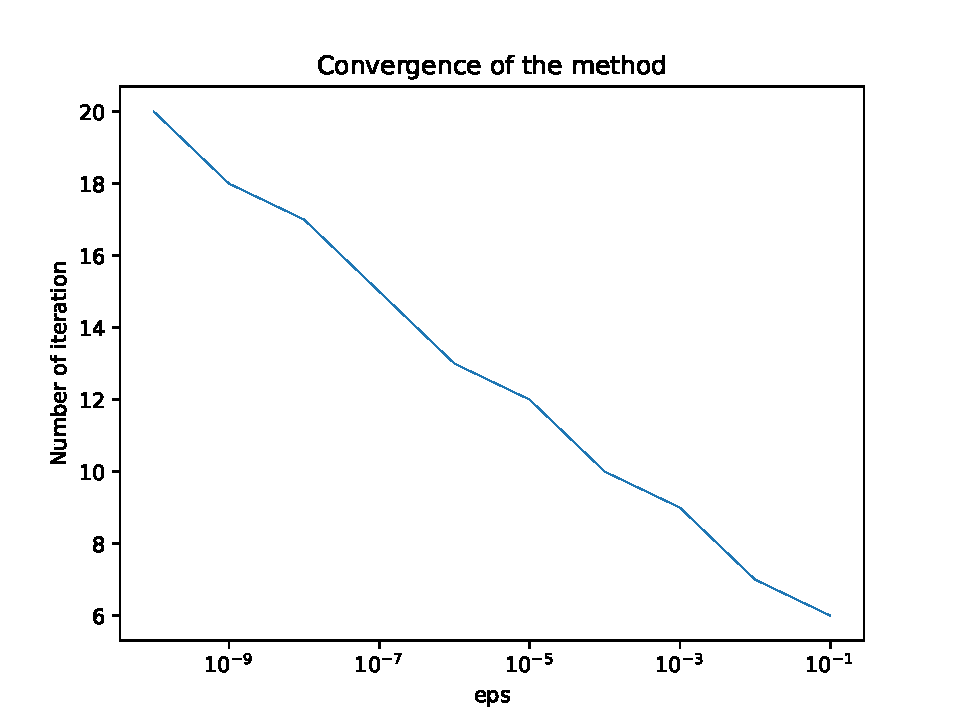
\includegraphics[scale=0.75]{1.pdf}

Из данного графика можно сделать вывод, что при увеличении количества итераций точность вычислений увеличивается

\subsection{Влияние шага на точность вычислений}

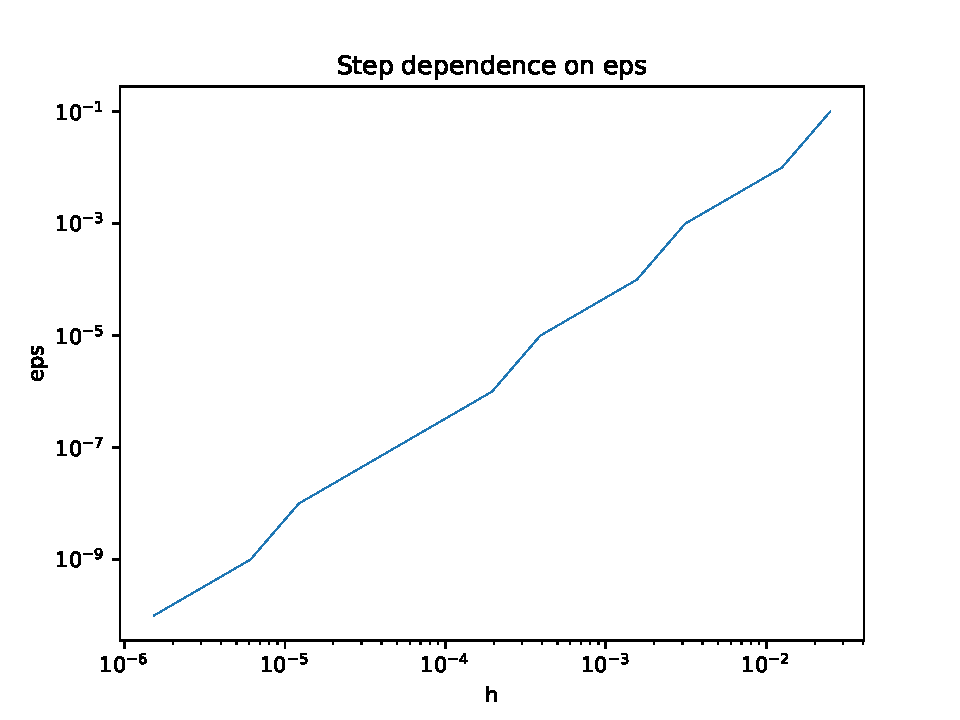
\includegraphics[scale=0.75]{2.pdf}

Из данного графика можно сделать вывод, что для достижения большей точности нужно уменьшать шаг равномерной сетки.

\subsection{Влияние ошибки исходных данных на решение}

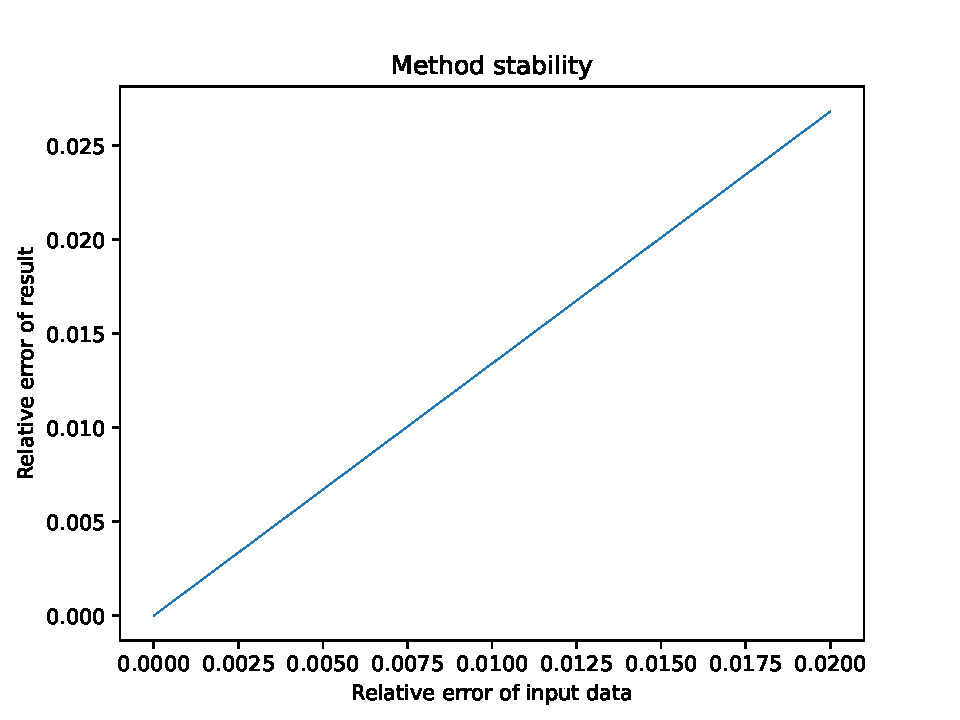
\includegraphics[scale=0.75]{3.pdf}

Из данного графика можно сделать вывод, что при увеличении ошибки в исходных данных ошибка вычислений увеличивается. Данная задача является устойчивой, т.к. ошибка входных данных и ошибка результата имеют одинаковый порядок.

\section{Краткие выводы}

На основе полученных результатов можно сделать вывод о том, что при увеличении количества итераций и шага разбиения равнмоерной сетки погрешность результата уменьшается. Также можно сделать вывод о том, что если в исходные данные вносить ошибки, то при ее увеличении будет увеличиваться и ошибка результата. Данная задача является устойчивой, т.к. ошибка входных данных и ошибка результата имеют одинаковый порядок.

\end{document}
